% ==================================================================================================================================
% Introduction

\minitoc  % Affiche la table des matières pour ce chapitre

Depuis le lycée, nous avons défini l'intégrale avec la définition de Riemann (ou Darboux pour les plus chauvins d'entre nous).

\begin{remark}[Intégrale de Riemann]
    Soit $[a,b] \subseteq \R $ et soit $f$ une fonction continue par morceaux sur $[a,b]$. On peut alors définir :
        \[ \int_{a}^{b} f = \int_{a}^{b} f(x) dx \]
\end{remark}

Cependant cette définition se heurte à quelques problèmes dont le plus important est le fait 
qu'elle ne peut pas se généraliser à des fonctions non définies sur $[a,b]$, non continues par morceaux ou à plusieurs variables.

Nous allons essayer dans les deux chapitres suivants de définir des outils et de nouvelles structures pour 
être capable d'intégrer de telles fonctions. 

% ==================================================================================================================================
% Espaces Mesurables

\section{Espaces Mesurables}

\subsection{Tribu Borélienne}

\begin{definition}[Tribu]
	Soit $X$ un ensemble. Une \emph{tribu} ou $\sigma$-algèbre sur $X$ est une partie 
	$\mathcal{B} \subseteq \mathcal{P}(X)$ telle que :
	\begin{itemize} 
		\item $ \emptyset \in \mathcal{B} $
		\item $ \forall A \in \mathcal{B}, A^c \in \mathcal{B} $
		\item Stabilité par union dénombrable : 
			$ \forall (A_i)_{i \in I}  A_i \in \mathcal{B}, \quad \forall i \in I, \quad \bigcup_{i \in I} A_i \in \mathcal{B} $
	\end{itemize}
Un élément de $\mathcal{B}$ est appelé une "partie mesurable" de $X$.
\end{definition}

\begin{definition}[Tribu Borélienne]
	Soit $E$ un espace topologique. La tribu borélienne est le plus petite tribu de $E$ contenant tous les ouverts de $E$. 
    On la note $\mathcal{B}_E$. Un borélien est un élément d'une tribu. 
\end{definition}

\begin{example} 
	$\mathcal{B}_\R$ est la \emph{tribu borélienne,} i.e la plus petite tribu contenant tous les ouverts de $\R$
\end{example} 

\begin{prop}[Intersection]
	Une sigma-algèbre est stable par \emph{intersection dénombrable}.
\end{prop} 

Le concept de tribu va nous servir plus tard lors de l'intégration de fontions pour "découper" leur domaine de 
définition de son ensemble de départ et permettre leur intégration. 

\begin{definition}[Espace Mesurable]
    Soit $X$ un ensemble et $ \mathcal{B}$ une tribu sur cet ensemble. 
    On appelle \emph{espace mesurable} le couple $(X, \mathcal{B})$.
\end{definition}

\subsection{Fonctions Mesurables} 

Dans toute la suite de ce cours, on se place dans un espace mesurable quelconque $(X, \mathcal{B})$. 


\begin{definition}[Fonction Mesurable]
    Soient $(X, \mathcal{B})$ et $(X', \mathcal{B}')$ deux espaces mesurables. 
	On dit que $f : (X,\mathcal{B}) \longrightarrow (X',\mathcal{B}')$ est mesurable ssi :
		\[ \boxed{ \forall A \in \mathcal{B}', \quad f^{-1}(A) \in \mathcal{B} } \]
    On notera $ \overline{\mathcal{M}(X)}$ l'ensemble des fonction mesurables étendues et 
     $ \overline{\mathcal{M}_+(X)}$ l'ensemble des fonction mesurables positives étendues. 
\end{definition}

\begin{remark}
	On appelle \emph{fonction borélienne} toute fonction mesurable au sens de la tribu borélienne. 
\end{remark}

\begin{prop}[Mesurabilité]
    Quelques propriétés (utiles) sur la mesurabilité :
    \begin{itemize} 
        \item La mesurabilité est stable par composition.
        \item La mesurabilité est stable par recollement dénombrable i.e :
            \[ f : X \longrightarrow X' \quad X = \bigcup_{n \in \N} A_n \text{ parties deux à deux disjointes mesurables} \]
            \[ \text{ si } \forall n \in \N, \quad f \restriction_A \text{ est mesurable} \]
        \item Toute fonction continue $f : E \longleftarrow E'$ ou $E$ et $E'$ sont deux espaces topologiques est mesurable.
        \item Toute fonction continue est mesurable (réciproque généralement fausse)
        \item De même, toute fonction continue par morceaux est mesurable.
    \end{itemize}
\end{prop}

Une fonction mesurable sera donc une fonction qui respecte la structure d'un espace mesurable et notamment 
sa tribu. 

\subsection{Fonctions mesurables réelles ou complexes} 

\begin{prop}[Lien Mesurabilité et Indicatrice]
	Soit $X$ un ensemble et $A \subseteq X$ et soit $1_A$ la fonction indicatrice de $A$.
    Alors : 
		\[ \forall A \subseteq X, \quad A \in \mathcal{B} \Longleftrightarrow 1_A \in \mathcal{M}_+(X) \] 
\end{prop}

Cette proposition établit un lien fondamental entre la mesurabilité des ensembles et celle des fonctions.
Elle permet notamment d’identifier les ensembles mesurables comme ceux dont l’indicatrice est mesurable.
Cela justifie l'étude des fonctions indicatrices comme briques de base pour construire des fonctions mesurables.

\begin{theorem}[Stabilité]
	La mesurabilité est stable par opérations algébriques élémentaires (+,.).
\end{theorem} 

\begin{theorem}[Convergence Simple]
	Soit $(f_n)$ une suite de fonctions à valeurs dans $\mathcal{M}(X)$ qui converge simplement vers une fonction $f : X \longrightarrow \C$ 
		\[ \text{i.e } \forall x \in X, \lim_{n\to\infty} f_n(x) = f(x) \]
		% \[ \Longleftrightarrow \forall \varepsilon > 0, \forall x \in X, \exists n_0 \in \N, \forall n \geq n_0, \lvert f_n(x) - f(x) \rvert < \varepsilon \] 
Alors : $f \in \mathcal{M}(X)$ 
\end{theorem} 

\begin{theorem}[Stabilité par inf/sup]
	Soit $(f_n)_{n\in\N} \in (\overline{\mathcal{M}_+(X)})^\N$ une suite de fonctions, on a :
	\[ \sup_{n\in\N} f_n : 
		\begin{cases}
			X &\longrightarrow \overline{\R_+} \\
			x &\longmapsto \sup_{n\in\N} f_n(x) = \sup \{ f_n(x) : n \in \N \}
		\end{cases} \]
Alors :  $\sup_{n\in\N} f_n \in \overline{\mathcal{M}_+(X)}$
\end{theorem}

\begin{definition}[Fonction Etagée]
	Soit $(X,\B)$ un espace mesurable. Une fonction $e : X \rightarrow \R$ est dite étagée si :
		\begin{itemize}
			\item $e \in \M_\R(X)$
			\item $e$ prend un nombre fini de valeurs distinctes 
		\end{itemize}
\end{definition}

\begin{prop}[Fonction étagée et parties mesurables]
	$e$ est une fonction étagée ssi $e$ est une combinaison linéaire d'indicatrices de parties mesurables.
\end{prop}

\begin{theorem}[Fondamental de l'intégrale de Lebesgue]
	si $f \in \overline{\M_+(X)}$, alors il existe une suite de fonctions croissantes étagées $(e_n)_{n\in\N}$ telle que :
		\[ \boxed{ (e_n) \quad \overset{\text{CS}}{\longrightarrow} \quad f} \] 
\end{theorem}

Les fonctions étagées sont donc les briques de base pour l'intégration de Lebesgue. En effet, grâce aux fonctions étagées 
définies sur un ensemble de boréliens, nous serons capables d'approcher très finement les fonctions à intégrer. 


% ==================================================================================================================================
% Mesures 

\section{Mesures}

\subsection{Définitions et généralités}

Soit $(X, \B)$ un espace mesurable.

\begin{definition}[Mesure]
    Une fonction sur $(X, \B)$ $ \mu : \B \longrightarrow \overline{\R_+} $ telle que :
    \begin{enumerate}
        \item $\mu (\emptyset) = 0 $
        \item $ \forall (A_n)_{n\in\N}$ suites de parties mesurables deux à deux disjointes :
            \[ \mu \left( \bigcup_{n\in\N} A_n \right) = \sum_{n=0}^{\infty} \mu (A_n) \]
    \end{enumerate}
    est appelée \textbf{mesure} sur l'espace $(X,\B,\mu)$, alors appelé espace mesuré.
\end{definition}

\begin{example}[Mesure de Comptage]
    Soient $X$ un ensemble et $\mathcal{B} = \mathcal{P}(x)$. On définit alors :
        \[ c :
            \begin{cases}
                \mathcal{P}(X) \longrightarrow \overline{\R_+} \\
                A \longmapsto \begin{cases}
                                    \infty \text{ si } A \text{ est infini }
                                    |A| \text{ sinon }
                                \end{cases}
            \end{cases}
        \] 
    est une mesure nommé \textbf{mesure de comptage}.
\end{example}

\begin{prop}[Mesures]
    Soit $(X,\B,\mu)$ un espace mesuré et $\mu$ sa mesure. Elle vérifie les propriétés suivantes :
    \begin{itemize}
        \item \textbf{Croissance :} La mesure est une fonction croissante i.e 

            \begin{minipage}{0.3\textwidth}
                \begin{tikzpicture}[scale=0.6]
                    % Dessin de l'ensemble B
                    \draw[thick] (-2,0) ellipse (3 and 2); % Patatoïde pour B
                
                    % Dessin de l'ensemble A (à l'intérieur de B)
                    \begin{scope}
                        \clip (-1.5,0) ellipse (2 and 1.5); % Clip pour hachurage uniquement dans A
                        \fill[pattern=north west lines, pattern color=gray] (-2,0) ellipse (3 and 2); % Hachurage de A
                    \end{scope}
                    \draw[thick] (-1.5,0) ellipse (2 and 1.5); % Contour de A
                
                    % Annotations
                    \node at (-3,1.5) {$B$};           % Annotation de B
                    \node at (-1.5,1) {$A$};           % Annotation de A
                    \node at (-4, -1) {$A \setminus B$}; % Annotation pour la partie A privé de B
                \end{tikzpicture}
            \end{minipage}%
            \hfill
            \begin{minipage}{0.55\textwidth}  % Largeur pour le texte
                $\forall A,B \in \B$ tels que  $A \subseteq B,$ on a  
                \begin{itemize}
                    \item  $\mu(A) \leq \mu (B)$
                    \item $\mu(B) = \mu(A) + \mu (B \setminus A)$
                \end{itemize}
            \end{minipage}

        \item \textbf{Convergence par union croissante :} Soit $(A_n)_{n\in\N}$ une suite croissante de parties mesurables
            \[ \text{ i.e } \forall n \in \N, A_n \subseteq A_{n+1}, \text{ alors } \mu \left( \bigcup_{n\in\N} A_n \right) = \lim_{n\to\infty} \mu(A_n) \] 
        \item \textbf{Convergence par intersection décroissante :} Soit $(A_n)_{n\in\N}$ une suite décroissante de parties mesurables de mesure finie
            \[ \text{ alors } \mu \left( \bigcap_{n\in\N} A_n \right) = \lim_{n\to\infty} \mu (A_n) \] 
    \end{itemize}
\end{prop}

\begin{definition}[Mesure Induite]
    Soit $A \subseteq C$ où $(X,\B,\mu)$ est un espace mesuré. On munit $A$ d'une structure d'espace mesuré $(A, \B_{\restriction _A}, \mu_A)$ où $\B_{\restriction _A}$ est la tribu induite.
    Alors $\mu_A$ est appelée mesure induite.
\end{definition}

\begin{definition}[Mesure Pondéré]
    Soit $\omega \in \mathcal{M}_+(X)$ et $(X, \mathcal{B},\mu)$ un espace mesuré. 

    Posons : $$ \mu_\omega = \omega \mu \quad \text{ où } \quad \mu_\omega : A \longmapsto \int_A \omega \; d \mu $$

    $\mu_\omega$ est alors appelée mesure pondérée par $\omega$. On a donc : 
        \[ f \in (X, \mathcal{B},\mu_\omega) \; \iff \; f \omega \in (X, \mathcal{B},\mu) \] 
\end{definition}

\begin{theorem}[Existence de la mesure de Lebesgue]
    Il existe une unique mesure sur $(\R, \B_\R)$ notée $\lambda$ telle que :
        \[ \boxed{ \forall a,b \in \R, a \leq b, \quad \lambda(]a,b]) = b-a } \] 
    Cette mesure est appelée \textbf{mesure de Lebesgue}. En partiulier, on a $ \lambda (\R) = \infty $ 
\end{theorem}

\begin{remark}
    $\lambda (\R) = \infty$ car :
        \[ R = \bigcup_{n \in \N} ]-n, n[ \text{ donc } \lambda (\R) = \lambda \Big( \bigcup_{n \in \N} ]-n, n[ \Big) = \lim_{n\to\infty} (2n) = \infty \] 
\end{remark}

\subsection{Parties négligeables et ensemble de Cantor}

\begin{definition}[Parties négligeables]
    Soit $A \in \B$ une partie mesurable, on dit que $A$ est une \textbf{partie néligable} ssi $\lambda (A) = 0 $.
    On dit aussi que $B \in \B$ est une \textbf{partie pleine} ssi $\lambda(B ^c) = 0 $.  On remarquera que toute partie dénombrable est négligeable.
\end{definition}

\begin{proof}
    Soit $A$ une partie dénombrable. On a $A = \bigcup_{x\in A} \{ x \}$ d'où :
        \[ \lambda (A) = \lambda \left( \bigcup_{x\in A} \{ x \} \right) = \lambda(x_1) + \dots + \lambda(x_n) = 0 \]
\end{proof}

\textbf{(?)} Existe-t-il une partie négligeable non dénombrable ?

\begin{example}[Ensemble de Cantor]
    Soit $(C_n)_{n\in N}$ une suite de fermés non vides décroissante. Posons $C = \bigcap_{n\in N} C_n$ un fermé non vide.
        \[ \text{Alors :  } \lambda (C) = \left( \frac{2}{3} \right) ^n \underset{n\to\infty}{\longrightarrow} 0 \]
    $C$ est donc négligeable mais on peut montrer que $C$ est en bijection avec $\{0,2\}^\N \simeq \R$ qui n'est pas dénombrable.
    Donc $C$ n'est pas dénombrable.

    \centering
    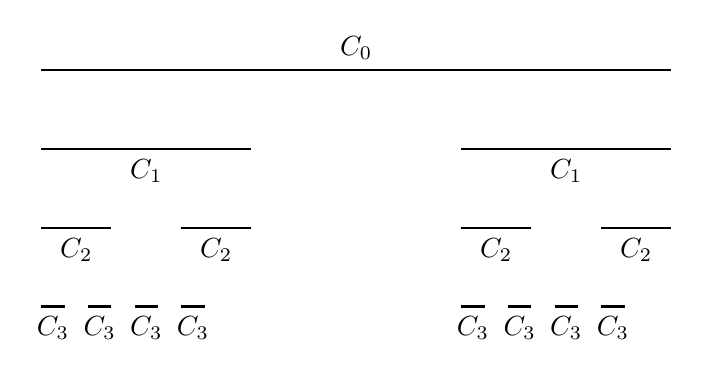
\begin{tikzpicture}[scale=1]
        % Définir la longueur initiale
        \def\length{8}
        \def\height{1}
        % Dessiner la première ligne (niveau 0)
        \draw[thick] (0, 0) -- (\length, 0) node[midway, above] {$C_0$};
        % Dessiner les lignes des niveaux suivants
        % Niveau 1
        \draw[thick] (0, -\height) -- (2.6667, -\height) node[midway, below] {$C_1$}; % 8/3
        \draw[thick] (5.3333, -\height) -- (8, -\height) node[midway, below] {$C_1$}; % 8/3
        % Niveau 2
        \draw[thick] (0, -2*\height) -- (0.8889, -2*\height) node[midway, below] {$C_2$}; % 8/9
        \draw[thick] (1.7778, -2*\height) -- (2.6667, -2*\height) node[midway, below] {$C_2$}; % 8/9
        \draw[thick] (5.3333, -2*\height) -- (6.2222, -2*\height) node[midway, below] {$C_2$}; % 8/9
        \draw[thick] (7.1111, -2*\height) -- (8, -2*\height) node[midway, below] {$C_2$}; % 8/9
        % Niveau 3
        \draw[thick] (0, -3*\height) -- (0.2963, -3*\height) node[midway, below] {$C_3$}; % 8/27
        \draw[thick] (0.5926, -3*\height) -- (0.8889, -3*\height) node[midway, below] {$C_3$}; % 8/27
        \draw[thick] (1.1852, -3*\height) -- (1.4815, -3*\height) node[midway, below] {$C_3$}; % 8/27
        \draw[thick] (1.7778, -3*\height) -- (2.0741, -3*\height) node[midway, below] {$C_3$}; % 8/27
        \draw[thick] (5.3333, -3*\height) -- (5.6296, -3*\height) node[midway, below] {$C_3$}; % 8/27
        \draw[thick] (5.9259, -3*\height) -- (6.2222, -3*\height) node[midway, below] {$C_3$}; % 8/27
        \draw[thick] (6.5185, -3*\height) -- (6.8148, -3*\height) node[midway, below] {$C_3$}; % 8/27
        \draw[thick] (7.1111, -3*\height) -- (7.4074, -3*\height) node[midway, below] {$C_3$}; % 8/27
    \end{tikzpicture}
\end{example}

\begin{definition}[Presque Partout]
    Une propriété $\mathcal{P}(X)$ qui dépend d'une variable $X$ variant dans une espace mesuré $(X,\B,\mu)$ est dite vraie "presque partout", noté (p.p) si 
        \[ \{ x \in X : \lnot \mathcal{P}(X) \} \text{ est négligeable } \] 
\end{definition}

\begin{example} Exemples de parties négligeables et propriétés vraies presque partout :
    \begin{itemize}
        \item  Soient $f,g \in \overline{\M_+(X)}$, on a :
            \[ f = g \text{ presque partout } \quad \Longleftrightarrow \quad \mu(\{x \in X : f(x) = g(x) \}) = 0 \] 
        \item $\mathbb{1}_\Q = 0$ p.p car $\Q$ est négligeable et $\R \backslash \Q$ est une partie pleine. 
    \end{itemize}
\end{example}

